%! TeX root = ./rims-smooth-paper.tex
\documentclass[./rims-smooth-paper.tex]{subfiles}
\begin{document}
\section{Implementation}
\label{sec:impl}
As an implementation language, we adopt a Haskell~\cite{haskell.org:2021tt}, a purely functional lazy programming language.
It has several virtues useful for our purpose:
\begin{enumerate}
\item It supports higher-order functions natively.
\item It is a lazy language, enabling us to treat \emph{infinite} structures.
\item The type-class mechanism in Haskell allows us to use function overloading in handy.
\end{enumerate}
For a general discussion on the advantages of using Haskell in computer algebra, we refer readers to Ishii~\cite{ISHII:2018ek}.

We follow the standard pattern in implementing ADs in Haskell: we use the function overloading to implement operations on types corresponding ADs.
This strategy is taken, for example, in Karczmarczuk~\cite{Karczmarczuk:2001ww}, Elliott~\cite{Elliott2009-beautiful-differentiation} and implemented in \texttt{ad} package~\cite{Kmett:2010aa}.
In Haskell, the \hask{Floating} type-class gives an abstraction over floating-point numbers that admit elementary functions, as excerpted in \Cref{lst:cls-floating}.
\begin{listing}[tbp]
\begin{code}
class Fractional a => Floating a where
  pi :: a
  exp :: a -> a
  log :: a -> a
  logBase :: a -> a -> a
  sin :: a -> a
  asin :: a -> a
  ...
\end{code}
\caption{The \texttt{Floating} class\label{lst:cls-floating}}
\end{listing}
\begin{listing}[tbp]
\begin{code}
  data AD a = AD a a deriving (Show, Eq, Ord)
  instance Floating a => Floating (AD a) where
    exp (AD f f') = AD (exp f) (f' * exp f)
    sin (AD f f') = AD (sin f) (f' * cos f)
    log (AD f f') = AD (log f) (f' / f)
    ...
\end{code}
\caption{The definition of \texttt{AD}\label{lst:def-AD}}
\end{listing}

For example, a simple forward-mode AD implemented as a dual number can be defined as in \Cref{lst:def-AD}.
The data-type \hask{AD} encapsulates a value of some univariate function and its first-order differential coefficient and calculates the result using the Chain Rule, using \hask{Floating}-operations on the coefficient \hask{a}.

So our goal is to implement \hask{STower n a} data-type conveying information of \emph{all} the higher-order derivatives of an $n$-variate smooth function on \hask{a}, which has \hask{Floating (STower n a)} instances for all \hask{Floating a} and $n$.

\begin{figure}[htbp]
  \centering
  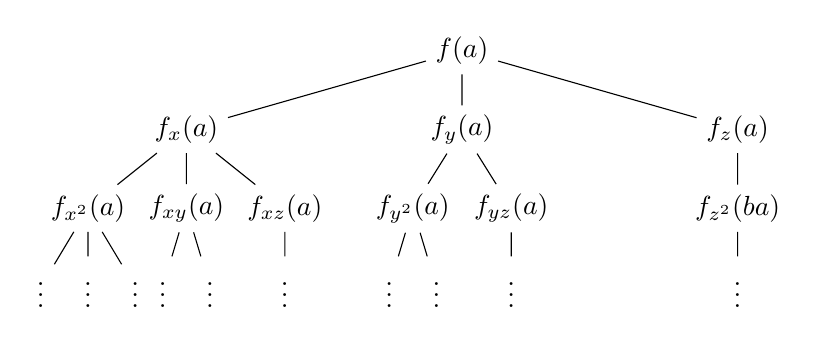
\begin{tikzpicture}[
    level/.style={level distance=1cm},
    level 1/.style={sibling distance=3.5cm},
    level 2/.style={sibling distance=1.25cm},
    level 3/.style={sibling distance=6mm}
    ]
    \newcommand{\ba}{\boldsymbol{a}}
    \node (fa) {$f(\ba)$}
      child{ 
        node (fxa) {$f_x(\ba)$}
          child { 
            node (fxxa) {$f_{x^2}(\ba)$}
            child {node{$\vdots$}}
            child {node{$\vdots$}}
            child {node{$\vdots$}}
          }
          child {
            node (fxya) {$f_{xy}(\ba)$}
            child {node{$\vdots$}} child {node{$\vdots$}}
          }
          child { 
            node (fxza) {$f_{xz}(\ba)$}
            child { node{$\vdots$} }
          }
      }
      child {
        node (fya) {$f_y(\ba)$}
        child { node {$f_{y^2}(\ba)$} child {node{$\vdots$}} child{ node{$\vdots$}} }
        child { node {$f_{yz}(\ba)$} child {node {$\vdots$}} }
      }
      child {
        node (fza) {$f_z(\ba)$}
        child {
            node {$f_{z^2}(ba)$}
            child { node {$\vdots$} }
        }
      };
  \end{tikzpicture}
  \caption{Ternary case\label{fig:tree}}
\end{figure}

\begin{listing}[tbp]
\begin{code}
data STower n a where
  ZS :: !a -> STower 0 a
  SS :: !a -> STower (n + 1) a -> STower n a -> STower (n + 1) a

liftSTower
  :: forall c n a. (KnownNat n, c a, forall x k. c x => c (STower k x) )
  => (forall x. c x => x -> x)
      -- ^ Function
  -> (forall x. c x => x -> x)
      -- ^ its first-order derivative
  -> STower n a
  -> STower n a
liftSTower f df (ZS a) = ZS (f a)
liftSTower f df x@(SS a da dus)
  = SS (f a) (da * df x) 
       (liftSTower @c f df dus)
\end{code}
\caption{Core definitions\label{lst:data-def}}
\end{listing}

\end{document}